\documentclass{IEEEtran}
\usepackage[utf8]{inputenc}
\usepackage[T1]{fontenc}
\usepackage[ngerman]{babel}
\usepackage[nolist]{acronym}
\usepackage{footnote}
\usepackage{algorithmic}
\usepackage{graphicx}
\usepackage[autostyle=true,german=quotes]{csquotes}
\usepackage{gensymb}
\usepackage{eurosym}
\usepackage{booktabs}
\usepackage{array}
\usepackage{subcaption}
\usepackage{todonotes}
\usepackage{microtype}
\usepackage{icomma}


\usepackage{hyperref}

\long\def\comment / *#1* /{}



% -----------------------------------------------------------------------------
% Visible TODO and FIXME markers
% -----------------------------------------------------------------------------
\newcounter{TODOCOUNT}
\newcommand{\TODO}[1]{\vspace{0.5em}\todo[inline, color=orange]{#1}\stepcounter{TODOCOUNT}}
\newcommand{\FIXME}[1]{\todo[size=\small, color=red]{#1}\stepcounter{TODOCOUNT}}
\AtEndDocument{
	\ifnum\value{TODOCOUNT}>0
		%\cleardoublepage
		\listoftodos
	\fi
}
% -----------------------------------------------------------------------------


\newcolumntype{x}[1]{>{\centering\arraybackslash\hspace{0pt}}p{#1}}



\begin{document}


\title{cowbusconfig -- Ansatz zur dezentralen Konfiguration von Gebäudeautomation}
\author{Patrick~Kanzler \and Michael~Zapf}
\date{\today}



\maketitle

\todo{nochmal über die Abkürzungen drüber gehen und schauen, wo man schön abkürzt (wenn der Text steht.)}

\begin{abstract}
    Um die Vorzüge intelligenter Haussteuerung einer breiten Masse zugänglich
    zu machen, müssen die System einfach handhabbar werden.
    Besonders die Konfiguration, also die Zuordnung von Sensoreignis zu
    Schaltaktion, muss einfach durchführbar und ebenso einfach anpassbar
    bzw. revidierbar sein. Diese Arbeit schlägt einen Ansatz vor,
    der in einem dezentralen Sensor-Aktor-Netzwerk eine einfache
    Konfigurationsmöglichkeit bieten soll.
    Einfache Wenn-Dann-Regeln werden in den Aktorknoten gespeichert und
    sind jederzeit auslesbar und änderbar.
    Im Betrieb wird dabei auf zentrale Komponenten verzichtet.
    Die eigentliche Konfiguration erfolgt per Webbrowser und ein Gateway,
    das den Zugang zum Sensor-Aktor-Netz ermöglicht.
\end{abstract}

\section{Einleitung}
    \enquote{Smart Home} ist ein Schlagwort, um das man im 21. Jahrhundert
    kaum noch herum kommt. Der moderne Mensch möchte sein Zuhause vernetzen.
    Vor allem in gewerblich genutzten Gebäuden ist es inzwischen üblich,
    auf die in der Vergangenheit übliche harte Verdrahtung von Sensoren und
    Aktoren -- zum Beispiel Lichtschalter und Leuchte -- zu verzichten
    und auf intelligente Einzelkomponenten zu setzen, die meist in einer
    Bustopologie verbunden sind. Der Vorteil liegt auf der Hand:
    Durch das Fehlen der festen und starren Zuordnung zwischen auslösendem
    Ereignis des Sensors (\emph{Lichtschalter gedrückt})
    und Wirkung des Aktors(\emph{Leuchte A an})
    können softwarebasiert Ursache-Wirkung-Beziehungen modelliert, evaluiert
    und korrigiert werden.

    Etablierte Systeme setzen dabei in der Regel auf eine
    Konfigurationssoftware, in der die teils komplexen Kommunikation- und
    Schaltvorgänge modelliert werden.
    Die einzelnen an den Bus angeschlossenen Komponenten werden häufig nur
    mit dem logischen Endergebnis konfiguriert,
    aus dem sich die ursprünglichen Absichten nicht mehr vollständig ableiten
    lassen.

    In dieser Arbeit beschäftigen wir uns mit dem Gedanken,
    Knoten in einem Gebäudeautomationsnetzwerk so konfigurierbar zu gestalten,
    dass die Konfiguration jederzeit mit minimalen Aufwand auslesbar
    und änderbar ist.
    Die Idee ist im Kontext der Vorlesung zum Thema \ac{DIY}
    von Dr.-Ing. Jürgen Eckert als studentisches
    Projekt entstanden und zielt deshalb auf einfachste Anforderungen ab.

\section{Verwandte Arbeiten}
    Gebäudeautomation wird inzwischen sowohl in der Praxis
    als auch in der Forschung erprobt. Hierbei konkurrieren verschiedene Systeme
    und Technologien, denen unterschiedlichste Paradigmen zugrunde liegen.
    Zur Veranschaulichung möchten wir hier ein System aus der Praxis betrachten,
    das auf dezentraler Kommunikation beruht,
    sowie einen Ansatz aus der Forschung,
    der einen zentralen Kommunikationsserver vorschlägt.

    \subsection{Europäischer Installationsbus (EIB) / KNX}
    Der unter der Abkürzung EIB bekannte Europäische Installationsbus
    ist ein offener Standard und nach subjektivem Empfinden das in der Praxis
    wohl meistgenutzte System in der Gebäudeautomation.
    Inzwischen wird er unter dem Namen KNX entwickelt und vertrieben.
    Es sind weltweit fast 7000 Produkte auf dem Markt\footnote{ KNX Association, \enquote{KNX -- Technologie -- Einführung}, \url{http://www.knx.org/knx-de/knx/technologie/einfuehrung/index.php}},
    die mit einer Twisted-Pair-Leitung verbunden werden
    (weitere Medien -- auch drahtlose -- sind verfügbar),
    über die Nachrichten direkt untereinander ausgetauscht werden\footnote{KNX Association, \enquote{KNX -- Technologie -- Kommunikationsmedien}, \url{http://
www.knx.org/knx-de/knx/technologie/kommunikationsmedien/index.php}}.

    Die Konfiguration der Schaltregeln etc. erfolgt nach der Installation
    der Komponenten durch einen Fachmann mithilfe von Software aus der
    ETS-Familie. Dabei handelt es sich um proprietäre Software,
    die von der KNX Association
    entwickelt und vertrieben wird\footnote{KNX Association,
        \enquote{KNX System Specifications -- Architecture}, 2001,
        \url{http://www.knx.org/media/docs/downloads/KNX-Standard/Architecture.pdf}}.

    KNX eignet sich besonders im Bereich großer Gebäude, in denen die
    elektrischen Systeme von einem Fachmann geplant, installiert und auch über
    Jahre hinweg gewartet werden. Ein entscheidender Nachteil von KNX ist,
    dass die Konfiguration, sobald sie einmal in die Steuergeräte geschrieben
    ist, nicht mehr ohne weiteres ausgelesen werden kann.
    Um die Konfiguration zu ändern (um zum Beispiel neue Komponenten einzufügen
    oder auch nur eine einfache Schaltregel anzupassen) wird jedes mal
    die ursprünglich erstellte Projektdatei aus der ETS-Software benötigt.

    \subsection{Zentrale skriptbasierte Steuerung}
        T. Haenselmann et al. \cite{haenselmann2007skriptbasierte}
        beschreiben ein zentrales System, das weitgehend
        unabhängig von dem verwendeten Transportmedium ist.
        Sie schlagen eine drahtlose Kommunikation vor,
        der Kerngedanke jedoch, auf den wir uns hier beziehen werden,
        gilt jedoch medienunabhängig.
        Der grundlegende Ansatz besteht in der Einrichtung eines zentralen
        Servers, bei dem alle Nachrichten des Systems zusammenlaufen.
        Sensoren melden ihre Messwerte an diesen, der dann Schaltnachrichten
        an die Aktoren sendet.
        Die Entscheidung, welche Aktionen ausgelöst werden, trifft der Server
        mithilfe von Skripten, die der Benutzer hinterlegt.
        Diese Skripte können auch über eine Weboberfläche erstellt und
        verwaltet werden.

        Der Nachteil des Ansatzes liegt auf der Hand:
        Sobald alle Schaltaufgaben von einem zentralen Punkt aus bearbeitet
        werden entsteht eine Abhängigkeit des gesamten Systems von einer
        einzelnen Komponente.
        Fällt diese aus, funktioniert kein einziger Lichtschalter mehr.

    %\cite{drossos2013ansteuerung}
    %\cite{kuntz6servicecast}
    %\cite{kuntz2011dienstbasierte}

\section{Ansatz}
    Inspiriert von Haenselmann et al. \cite{haenselmann2007skriptbasierte}
    möchten wir ein System vorschlagen,
    das ebenso über eine einfache Weboberfläche konfiguriert werden kann.
    Der Benutzer kann dort einfache Wenn-Dann-Regeln anlegen, bearbeiten und
    löschen, die das Verhalten der Aktoren in Abhängigkeit von Sensorereignissen
    festlegen.

    Der grundlegende Unterschied im Ansatz besteht jedoch darin,
    dass wir auf eine zentrale Kommunikationseinheit verzichten.

    \subsection{Voraussetzungen, Annahmen}
        Wir gehen davon aus, dass uns ein paketvermitteltes Netz vorliegt,
        in dem alle Teilnehmer eindeutig adressierbar sind.

        Als Test- und Referenzumgebung dient uns der \emph{cowbus}.
        Dabei handelt es sich um ein studentisches Projekt,
        das sich zum Ziel gesetzt hat,
        eine kostengünstige und einfach nachzubauende Plattform zu schaffen,
        die einen Einstieg in den Arbeits- und Forschungsbereich des
        \enquote{Smart Home} bzw. \enquote{Connected Home} ermöglichen soll.
        Der Nachrichtenaustausch erfolgt dabei drahtlos über eine
        $2,4$\,GHz-Funkverbindung als geflutete Broadcasts in einer
        Mesh-Topologie.
        Eine umfangreichere Beschreibung des Projektes
        steht auf der Projektseite des Lehrstuhles zur Verfügung,
        die Daten des Projekts sind bei GitHub
        verfügbar\footnote{Dokumentation siehe: \url{http://www7.cs.fau.de/de/wp-content/uploads/sites/2/2014/08/projektdoku_cowbus.pdf}; Projekt siehe: \url{https://github.com/michz/diy14bus}.}.

    \subsection{Idee}
        Da \textbf{Sensoren} häufig höhere Anforderungen an den Energieverbrauch
        stellen, sollen sie in dem System \enquote{dumm} sein.
        Sie erarbeiten sich also kein Wissen über die anderen Netzwerkkomponenten
        und reagieren nicht, sondern agieren ausschließlich.
        Das ermöglicht uns sie die meiste Zeit in Energiesparmodi zu betreiben
        und nur dann aufzuwecken, wenn sie selbst ein Ereignis auslösen,
        zum Beispiel wenn der Benutzer einen Taster betätigt.

        \textbf{Aktoren} hingegen sind häufig mit stabilen Energiequellen
        ausgestattet, da sie meist gewisse Lasten schalten.
        Als Beispiele wären Leuchten, Jalousiemotoren oder auch Ventilatoren
        zu nennen.
        Daher bietet es sich an, logische Verknüpfungen hier vorzunehmen.
        Aktoren empfangen also die Ereignisse, die von Sensoren generiert werden.
        Diese sind im einfachsten und üblichsten Fall einfach die Zustände
        der Sensoren, zum Beispiel eine Temperatur oder eine Schalterposition.
        Auf Basis dieser Ereignisse treffen Aktoren dann mithilfe von
        Regeln (siehe unten) Entscheidungen und führen Schaltaktionen aus.

        Ein \textbf{Gateway} verbindet das Sensor-Aktor-Netz mit einem
        vorhandenen herkömmlichen \ac{LAN} oder \ac{WLAN}.
        Es muss mit einem Funkmodul ausgestattet sein,
        um mit den Sensoren und Aktoren zu kommunizieren,
        und mit einer \ac{LAN}- bzw. \ac{WLAN}-Schnittstelle.
        Es stellt einen Webserver zur Verfügung,
        der die Konfigurationswebseite im \ac{LAN}- bzw. \ac{WLAN} anbietet.

        Die eigentliche \textbf{Konfiguration} der Aktoren wird dann
        über ein webfähiges Gerät vorgenommen,
        das über das \ac{LAN} bzw. \ac{WLAN} die
        Konfigurationswebseite des Gateways anzeigt.
        Dabei werden Konfigurationsnachrichten \enquote{in-band} gesendet,
        also neben den Nutzdaten auf demselben Funkkanal:
        Die Aktoren erkennen sie an speziellen Nachrichtentypen
        und aktualisieren ihre interne Regeltabelle anhand der empfangenen
        Konfigurationspakete.

        Wie bereits angeklungen basiert die Konfiguration auf \textbf{Regeln},
        auf die im Abschnitt \ref{subsec:regeln} genauer eingangen wird.
        Jeder Aktorknoten muss eine oder mehrere Regeln speichern,
        auf Anfrage auslesen und rückmelden sowie löschen können.
    \begin{figure*}
        \centering
        \begin{subfigure}{1\columnwidth}
            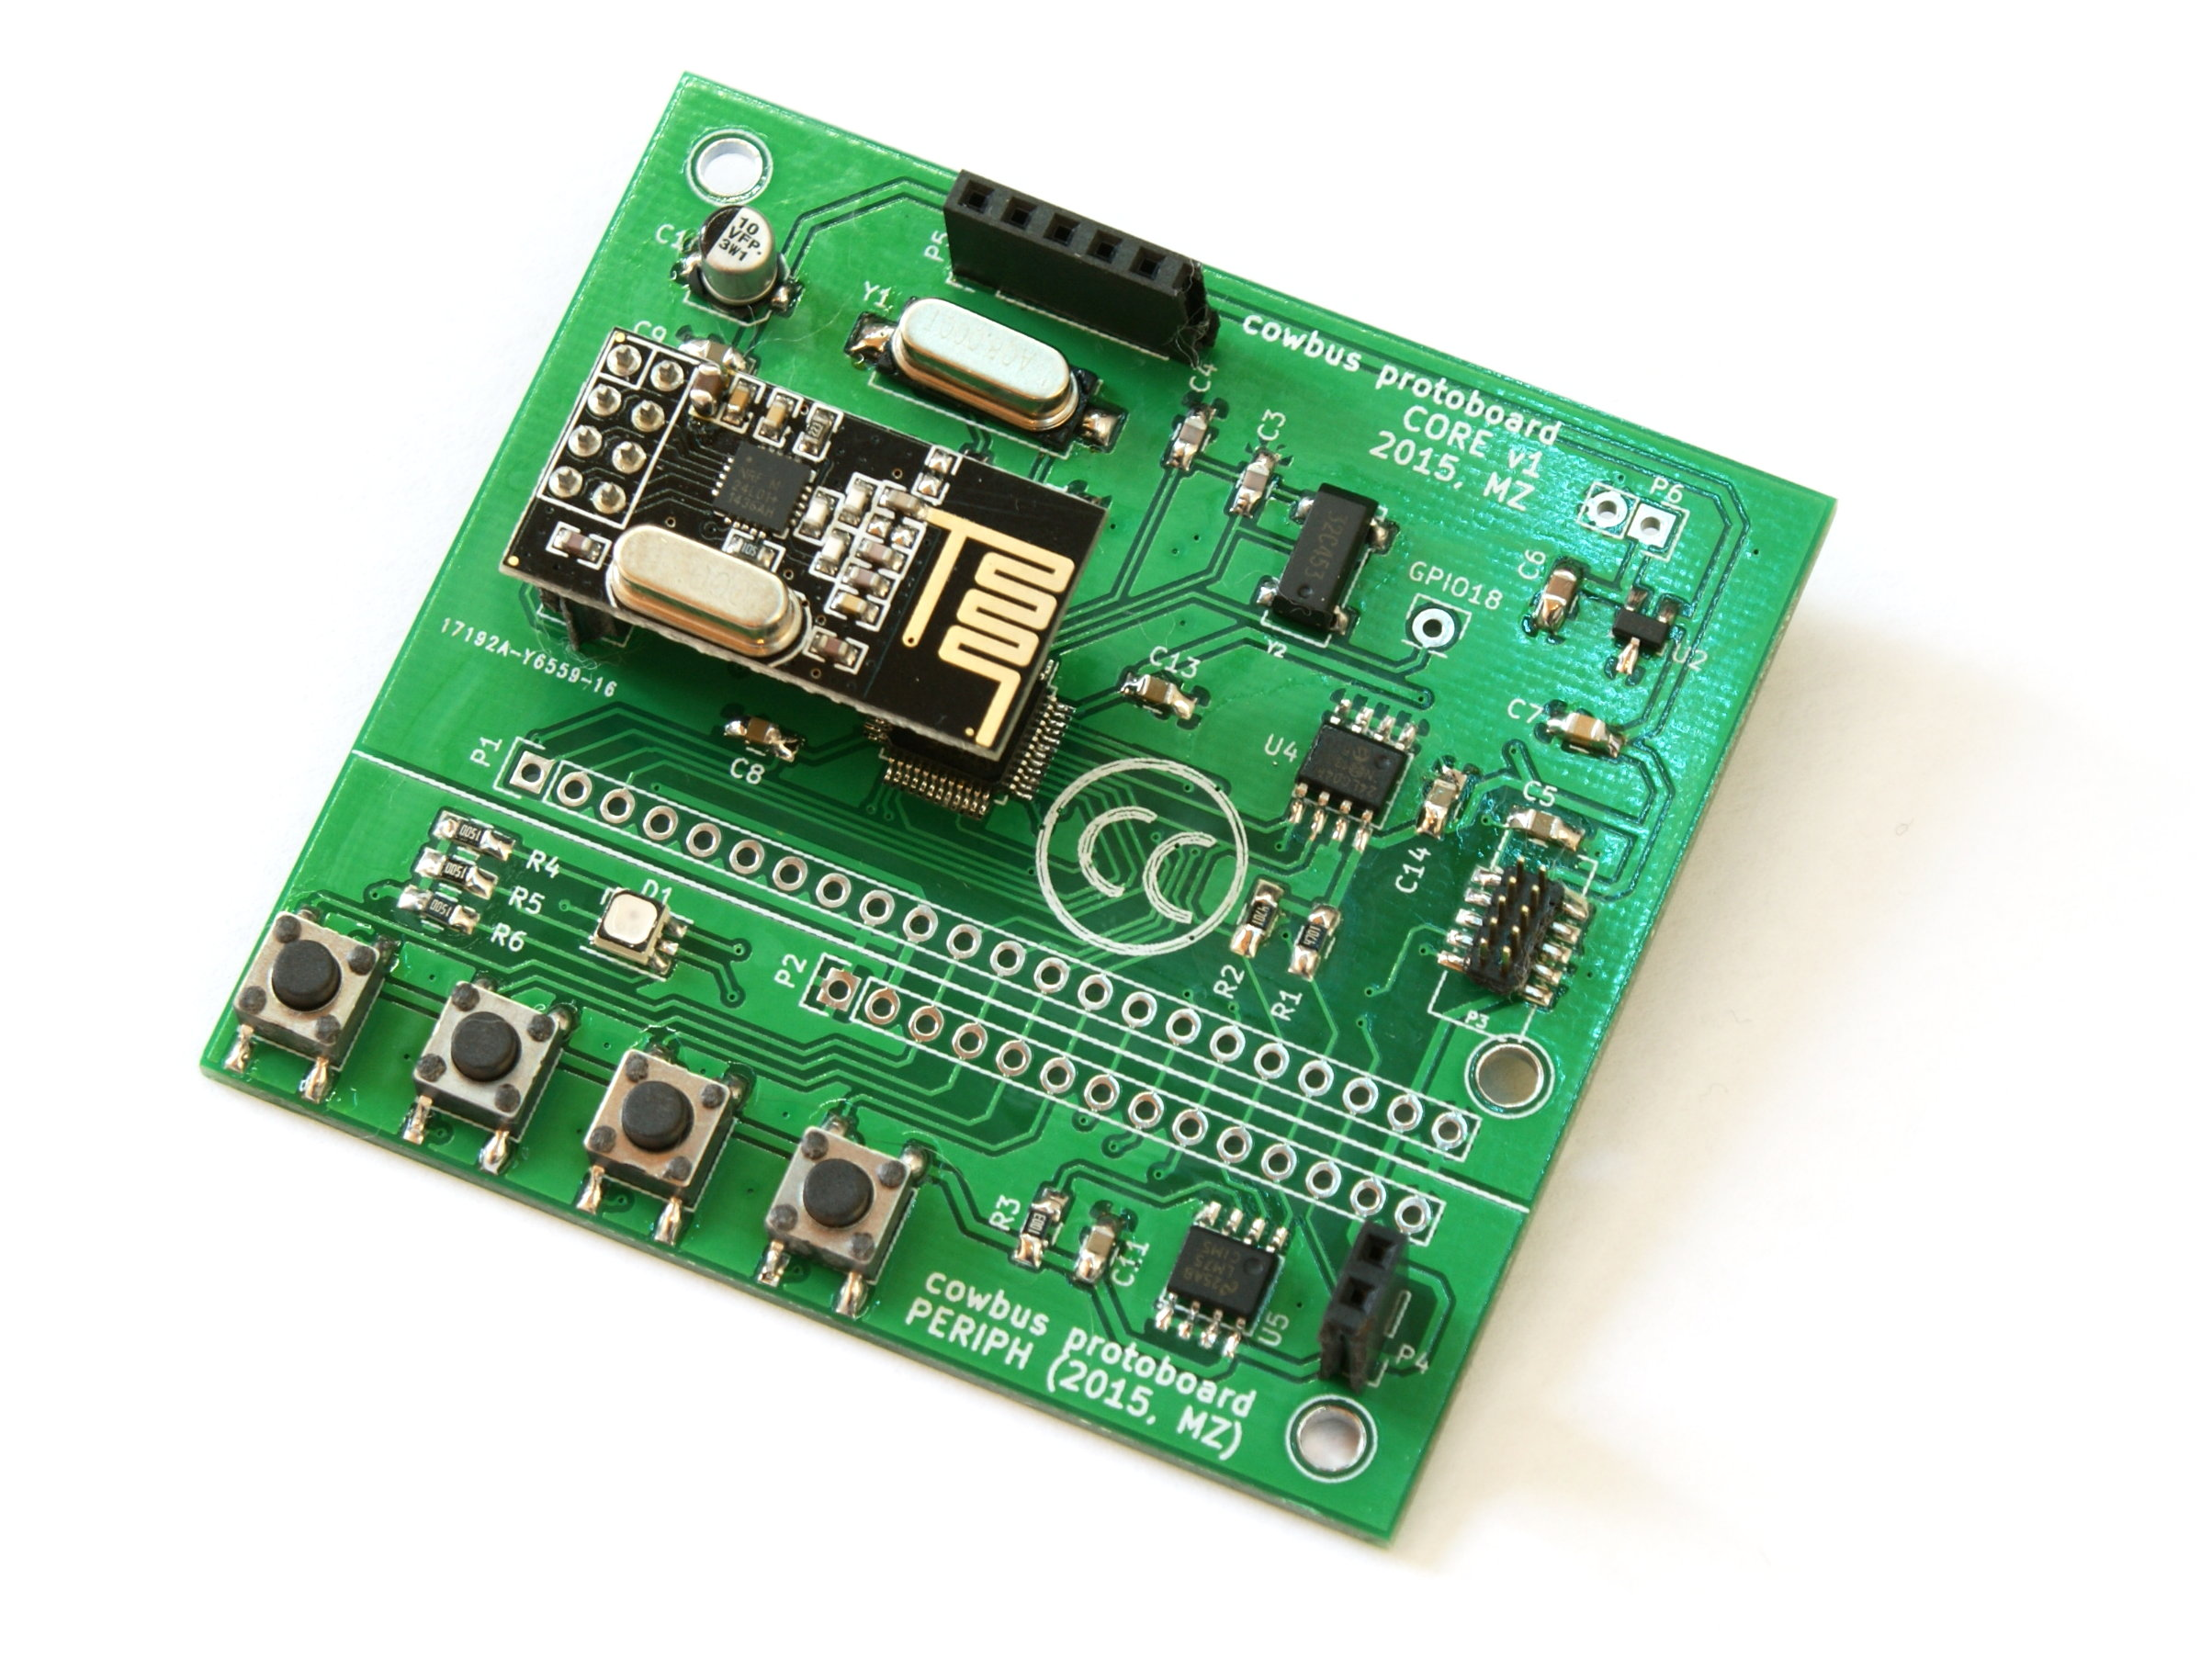
\includegraphics[width=\columnwidth]{img/img-cowbus-proto}
            \caption{Sensor- sowie Aktorknoten werden durch cowbus-Prototyping-Boards realisiert.}
            \label{subfig:proto}
        \end{subfigure}\hfill
        \begin{subfigure}{1\columnwidth}
            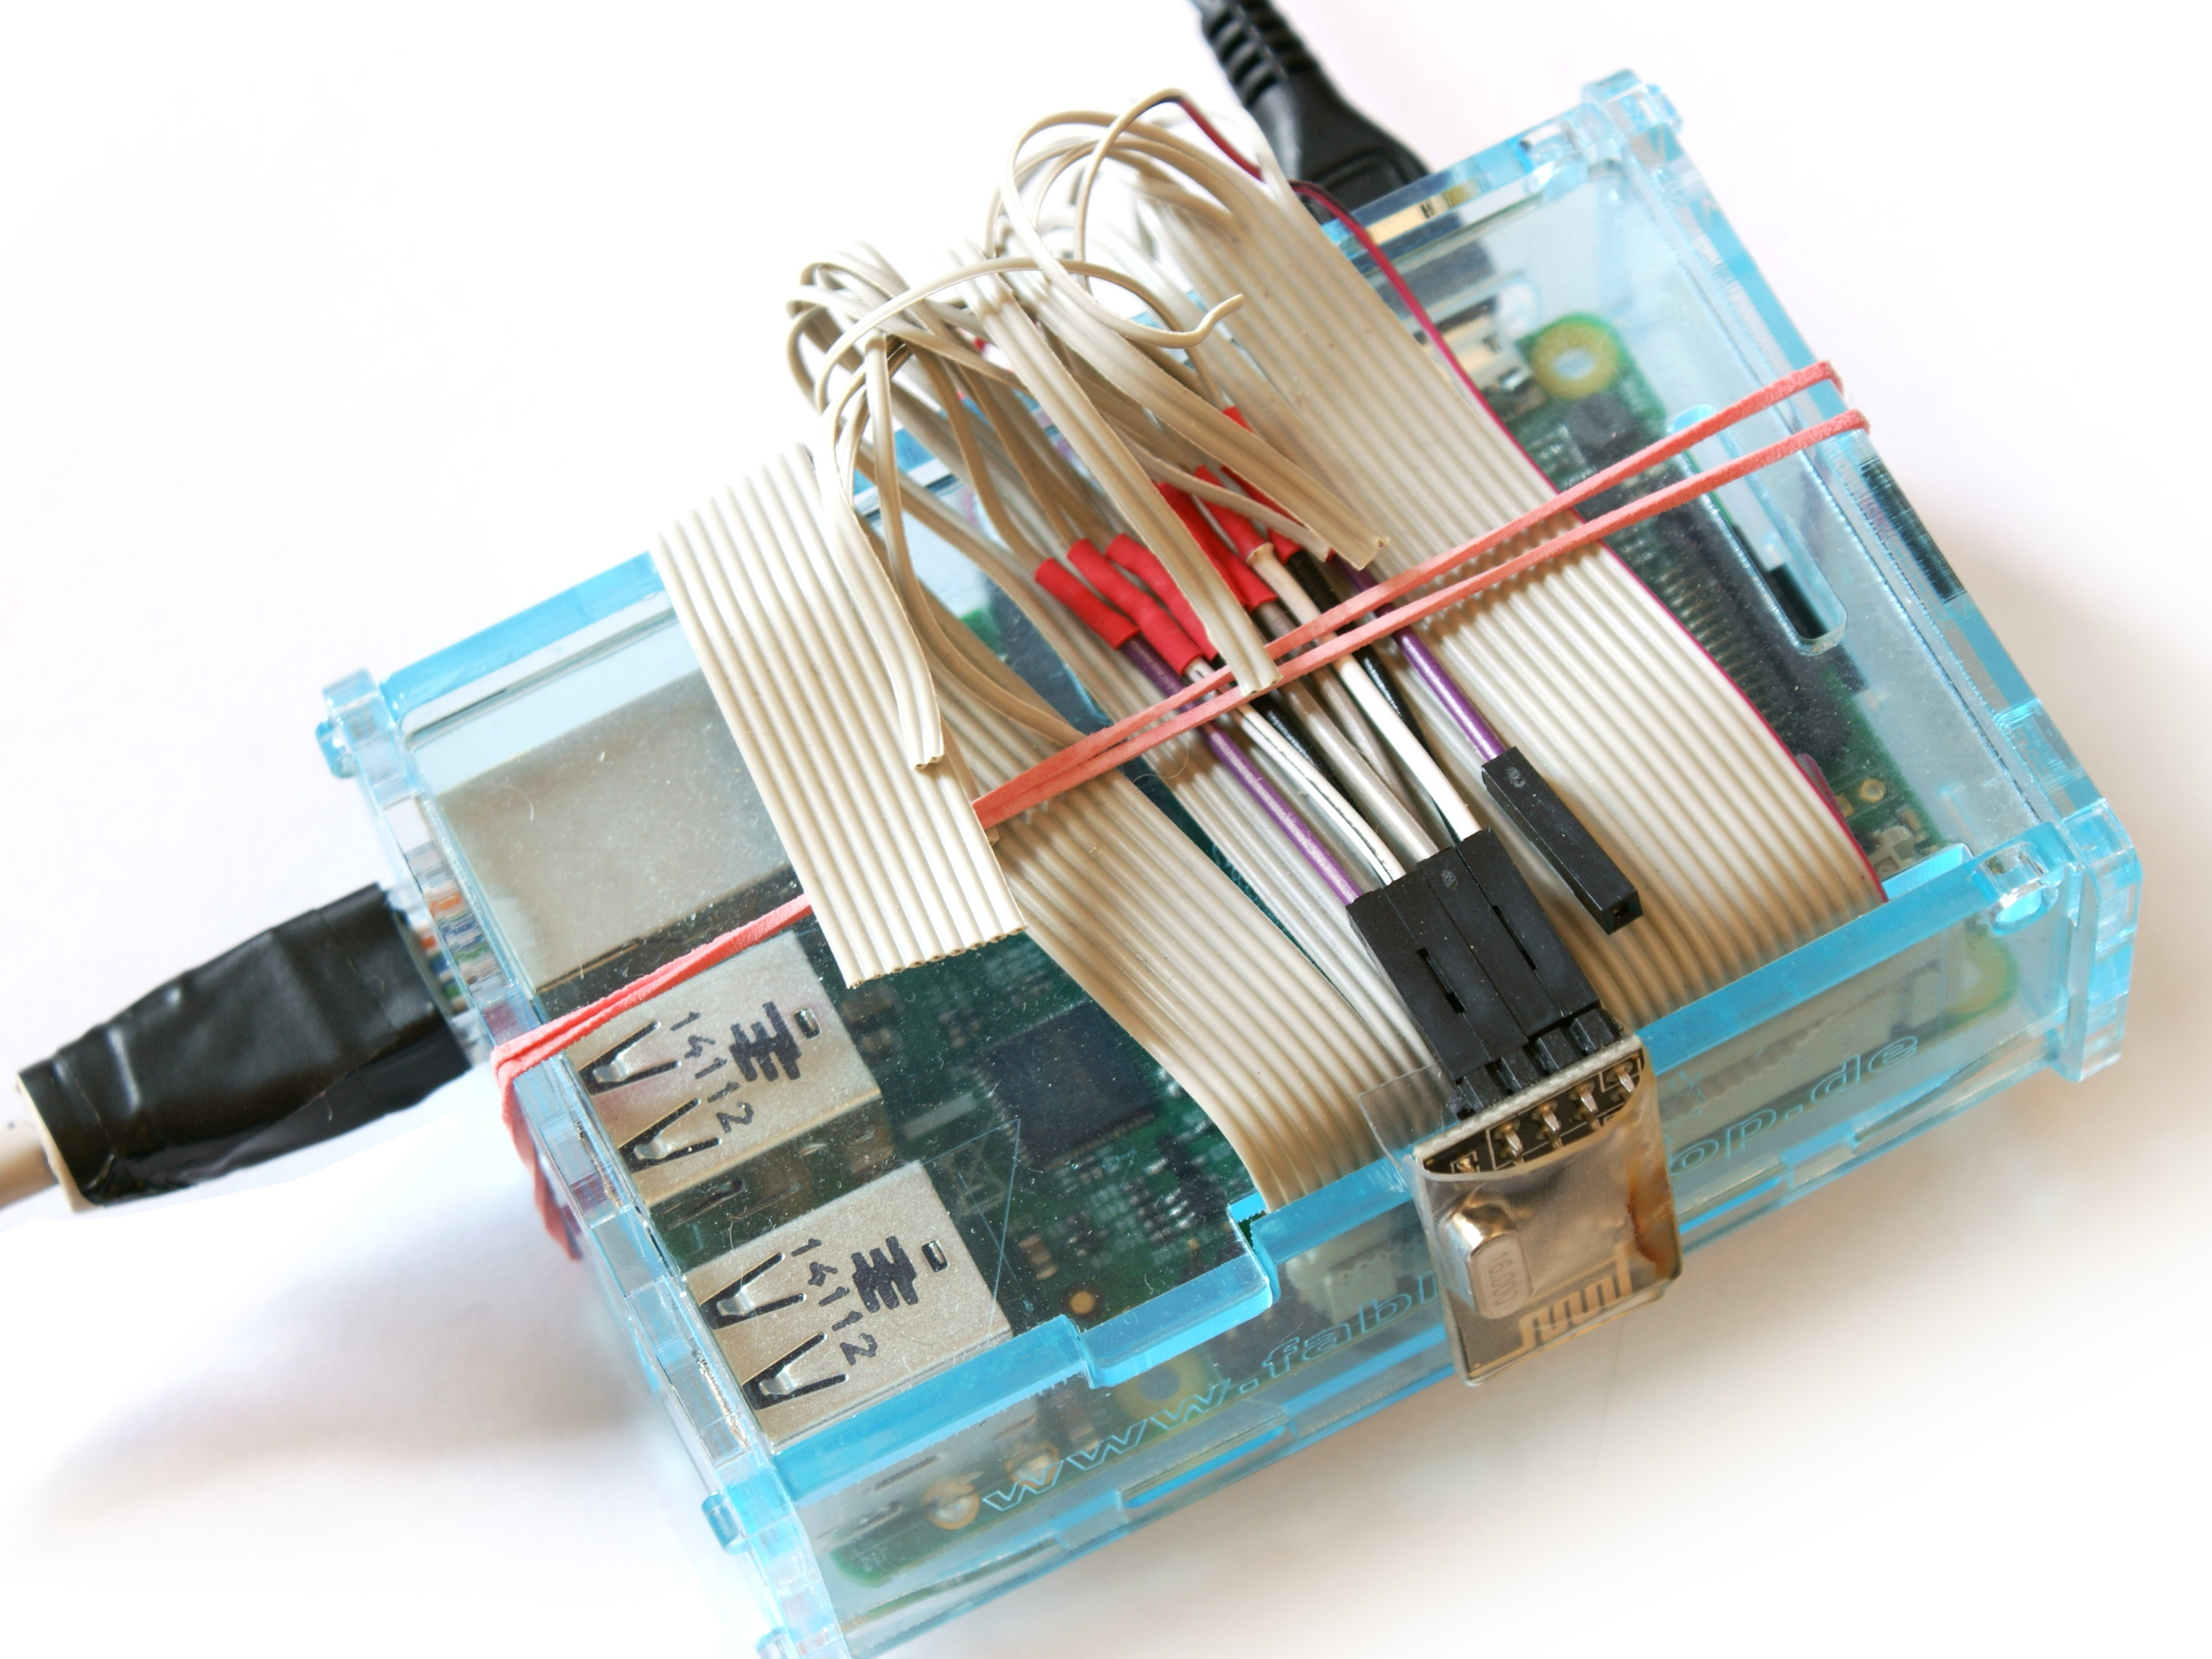
\includegraphics[width=\columnwidth]{img/img-pi-rf}
            \caption{Die Funktion des Gateways wird von einem Raspberry Pi übernommen.}
            \label{subfig:pi}
        \end{subfigure}\hfill
        \caption{Komponenten der Testumgebung}
        \label{fig:comp}
    \end{figure*}

    \subsection{Regeln} \label{subsec:regeln}
        Basis der Logik sind einfache Wenn-Dann-Regeln.
        Ein (Aktor)-Knoten kann theoretisch beliebig viele dieser Regeln befolgen.

        Eine Regel besteht aus mehreren Komponenten.
        Als Beispiel dient ein Temperatursensor,
        der einen Ventilator nur dann anschalten soll,
        wenn die Temperatur in einem bestimmten Intervall liegt.

        \begin{enumerate}
            \item Festgelegt wird, auf Pakete welcher \textbf{Adresse}
                die Regel zutrifft.
                Im Beispiel wäre dies die Adresse des Temperatursensors.
            \item Der \textbf{Operator} legt fest, wie der angegebene
                Schwellwert der Regel mit dem im Paket übertragenen Wert
                verglichen wird.
                Im Beispiel nutzen wir einen Intervalloperator.
            \item Verglichen wird jeweils mit dem bereits erwähnten
                \textbf{Schwellwert}. Wenn als Operator eine Intervallprüfung
                gewählt wird, müssen zwei Schwellwerte
                (ein oberer und ein unterer) angegeben werden.
                Im Beispiel wird das Intervall $[18;25]$ gewählt.
            \item Die \textbf{Aktion} gibt an, was der Aktor macht,
                wenn ein Paket eingetroffen ist, auf das die Regel zutrifft.
                Hier wird der Ventilator an- bzw. abgeschaltet.
        \end{enumerate}


        Soll ein Ventilator aktiviert werden, wenn der Wert eines Temperatursensors
        im Intervall $[18;25]$ liegt, könnten die zugehörigen Regeln wie folgt aussehen:

        \begin{center}
            \begin{tabular}{r|x{0.15\textwidth}|x{0.15\textwidth}}
                \toprule
                                        & \textbf{Regel 1} & \textbf{Regel 2} \\
                \midrule
                \textbf{Adresse}:       & \multicolumn{2}{c}{Sensoradresse} \\
                \textbf{Operator}:     & \enquote{$\leq \geq$} & \enquote{nicht $\leq \geq$} \\
                \textbf{Schwellwert A}: & \multicolumn{2}{c}{18} \\
                \textbf{Schwellwert B}: & \multicolumn{2}{c}{25} \\
                \textbf{Aktion}:        & \enquote{Ventilator an}  & \enquote{Ventilator aus} \\
                \bottomrule
            \end{tabular}
        \end{center}

    \subsection{Konfigurationsnachrichten}
        Um die Konfiguration jederzeit auslesbar und änderbar zu gestalten
        sind folgende Nachrichtentypen vorgesehen:

        \begin{itemize}
            \item \textbf{LIST} fordert einen Knoten auf, seine Konfiguration
                auszugeben.
            \item \textbf{ADD} fügt einem Knoten eine Regel hinzu.
            \item \textbf{DELETE\_ONE} löscht eine Regeln auf einem Knoten.
            \item \textbf{DELETE\_ALL} löscht alle Regeln auf einem Knoten.
            \item \textbf{DELETE\_ADDR} löscht alle Regeln auf einem Knoten mit
                einer bestimmten Quelladresse.
        \end{itemize}



\section{Evaluation}
    Das Testnetzwerk besteht aus drei Komponenten:
    \begin{itemize}
        \item Als \textbf{Sensor} dient ein Taster auf einem
            cowbus-Prototyping-Board (Abb. \ref{subfig:proto}).
        \item Eine \ac{LED} ebenfalls auf einem cowbus-Prototyping-Board dient
            als \textbf{Aktor},
        \item Die Rolle des \textbf{Gateways} übernimmt ein Raspberry Pi,
            der um ein Funkmodul erweitert wurde (Abb. \ref{subfig:pi}).
            Alternativ wäre auch denkbar ein USB-Dongle zu entwickeln,
            das ebenfalls um ein Funkmodul verfügt und an einen beliebigen
            Rechner angeschlossen werden kann.
    \end{itemize}

    Der vorgestellte Ansatz funktioniert in diesem kleinen Maßstab sehr gut.
    Einfache Schaltregeln lassen sich damit ohne großen Aufwand
    realisieren. Werden die Regeln in den Knoten persistent gespeichert
    stellen diese eine ähnlich stabile und dauerhafte Konfiguration dar, wie
    sie die eingangs erwähnten Systeme bieten.


\section{Zusammenfassung und Ausblick}
    Mit cowbusconfig haben wir einen Ansatz zur einfachen Konfigurierbarkeit
    von Sensor-Aktor-Netzwerken im Hausautomationsbereich vorgestellt.
    Die Besonderheit gegenüber bisher üblichen oder erforschten Ansätzen ist
    dabei die Möglichkeit auf zentrale \enquote{Logik}-Komponenten
    zu verzichten und trotzdem die Konfiguration wiederauslesbar und
    änderbar zu gestalten.
    Damit ist es möglich, auf einfache Art und Weise neue Komponenten in das
    System zu integrieren und entsprechende Schaltregeln hinzuzufügen bzw.
    anzupassen, ohne das komplette System neu einstellen zu müssen.

    Offen bleibt jedoch die Frage, wie komplexere logische Abhängigkeiten
    dargestellt werden können.
    Zu Beispiel wäre es interessant eine Aktion nur dann auszuführen,
    wenn ein bestimmtes Ereignis über einen bestimmten Zeitraum mehrfach ohne
    widersprüchliche \enquote{Ausreißer} auftritt.
    So könnte es im Beispiel des Ventilators sinnvoll sein, diesen nur zu
    aktivieren, wenn der Temperaturwert über eine Minuten lang konstant über
    dem Schwellwert liegt, um versehentliche Schaltaktionen aufgrund von
    Messfehlern zu vermeiden, die sowieso wenige Sekunden später revidiert
    würden. Mögliche Ansätz reichen von der Pufferung von
    Werten innerhalb des Aktors bis hin zu autonomen Aggregatorknoten,
    die nichts weiter machen als Ereignisse zu beobachten und daraus
    neue Ereignisse zu generieren.



\section*{Implementierungen}
    Beispielhardware und -code sind unter freien Lizenzen im
    cowbus-GitHub-Projekt verfügbar:

    \url{https://github.com/michz/diy14bus}

\section*{Danksagung}
    Wir möchten uns bei Dr.-Ing. Jürgen Eckert bedanken,
    der uns mit der Lehrveranstaltung
    \enquote{DIY: Personal Fabrication}\footnote{\enquote{DIY: Personal Fabrication},
        Wintersemester 2014/2015, FAU,
        \url{http://www7.cs.fau.de/de/teaching/diy-2014w/}}
    und seiner persönlichen Unterstützung ermöglicht hat
    einen Einblick in die Forschung im Gebiet der modernen
    Sensor-Aktor-Netze zu gewinnen und dabei selbst sehr frei
    und selbstständig Erfahrungen zu sammeln.



%\section*{Abkürzungen}
\renewcommand{\IEEEiedlistdecl}{\IEEEsetlabelwidth{CSMA/CA}}
\begin{acronym}
    \acro{DIY}{Do-It-Yourself}
    \acro{LAN}{Local Area Network}
    \acro{LED}{Leuchtdiode}
    \acro{WLAN}{Wireless Local Area Network}
\end{acronym}
\renewcommand{\IEEEiedlistdecl}{\relax}% remember to reset \IEEEiedlistdecl

\comment / *
\listoffigures
\clearpage

\listoftables
\clearpage
* /


\bibliographystyle{IEEEtran}
\bibliography{IEEEabrv,projektdoku_cowbus}

\end{document}
